\documentclass[aspectratio=169]{beamer}
\usetheme{Madrid}
\usecolortheme{default}
\usepackage{graphicx}
\usepackage{hyperref}
\usepackage{multicol}
\setbeamertemplate{navigation symbols}{}
\graphicspath{{/root/github/e906-development/src/xsec_pT/RS57-70/}{/root/github/e906-development/src/CalculateDoubleDifferentialCrossSection/RS57-70/}}

\title{Measurement of Absolute Double Differential Cross-Section in Invariant Mass and $p_T$ Bins}
\author{Chatura Kuruppu}
\institute{SeaQuest Experiment (E906) \\ Fermi National Accelerator Laboratory}
\date{\today}

\begin{document}

\begin{frame}
    \titlepage
\end{frame}

\begin{frame}{Overview}
    
\begin{itemize}
    \setlength{\itemsep}{0.5em}
    \item Events from runs 2 and 3
    \item Kinematic Phase Space
    \item Event Selection Criteria
    \item Yield Distributions
    \item Efficiency Corrections
    \item Corrected Yields
    \item Corrected Yields Flask Subtracted
    \item Single Differential Cross-Section Plots
    \item Next Steps
\end{itemize}

\end{frame}

\begin{frame}{Input Files Used}
    
\textbf{Note:} Currently using all the runs saved in runs 2 and 3.

\vspace{0.2cm}
\tiny
\textbf{Currently using Harsha's ROOT files saved in:} \\
\texttt{/seaquest/users/harshaka/e906\_project/e906-root-ana/work\_gpvm/scripts/results\_runFinalTree/merged\_results\_e906\_mixing/:}
\begin{multicols}{2}
\begin{itemize}
    \item \texttt{merged\_RS57\_LH2\_1\_1138.root}
    \item \texttt{merged\_RS57\_LD2\_3\_1138.root}
    \item \texttt{merged\_RS57\_Empty\_2\_1138.root}
    \item \texttt{merged\_RS59\_LH2\_1\_465.root}
    \item \texttt{merged\_RS59\_LD2\_3\_466.root}
    \item \texttt{merged\_RS59\_Empty\_2\_466.root}
    \item \texttt{merged\_RS62\_LH2\_1\_1234.root}
    \item \texttt{merged\_RS62\_LD2\_3\_1237.root}
    \item \texttt{merged\_RS62\_Empty\_2\_1234.root}
    \item \texttt{merged\_RS70\_LH2\_1\_264.root}
    \item \texttt{merged\_RS70\_LD2\_3\_266.root}
    \item \texttt{merged\_RS70\_Empty\_2\_267.root}
\end{itemize}
\end{multicols}

\vspace{0.2cm}
\textbf{For RS67 using Abi's files saved in:} \\
\texttt{/seaquest/users/apun/e906\_projects/rs67\_merged\_files/:}
\begin{itemize}
    \item \texttt{merged\_RS67\_3089LH2.root}
    \item \texttt{merged\_RS67\_3089LD2.root}
    \item \texttt{merged\_RS67\_3089flask.root}
\end{itemize}
\normalsize

\end{frame}

\begin{frame}{Kinematic Phase Space}
    
\textbf{Kinematic Binning Definition:}
\begin{itemize}
    \item \textbf{Mass Bins (GeV):} [4.2, 4.5, 4.8, 5.1, 5.4, 5.7, 6.0, 6.3, 6.6, 6.9, 7.5, 8.7]
    \item \textbf{$p_T$ Bins (GeV):} [0.0, 0.32, 0.49, 0.63, 0.77, 0.95, 1.18, 1.8]
    \item \textbf{$x_F$ Bins:} [0.0, 0.85] with a fixed step width of 0.05.
\end{itemize}

\end{frame}

\begin{frame}{Event Selection Criteria}
    \footnotesize
    
\textbf{Dimuon Kinematics:}
\begin{itemize}
    \item $4.2 < \text{Mass} < 8.8$ GeV, $-0.1 < x_F < 0.95$, $0.05 < x_T \le 0.58$, and $|\cos\theta| < 0.5$.
    \item Vertex cuts: $-280 < dz < -5$, target/dump tracking separation criteria met.
    \item Transverse momentum bounds: $|dp_x| < 1.8$, $|dp_y| < 2.0$, and $dp_x^2 + dp_y^2 < 5$.
\end{itemize}
\vspace{0.2cm}
\textbf{Track Quality \& Acceptance:}
\begin{itemize}
    \item $\chi^2_{\text{target}} < 15$, $\chi^2_{\text{dimuon}} < 18$, and $\chi^2/(\text{nHits}-5) < 12$.
    \item Hit requirements: nHits $> 13$ per track, $\text{nHits}_1+\text{nHits}_2 > 29$, St1 total $> 8$.
    \item Track vertex longitudinal limits: $-320 < z_v < -5$.
    \item A dynamic beam offset correction is applied to y-coordinates: offset is $1.6$ for runID $\ge 11000$ and $0.4$ otherwise.
\end{itemize}
\vspace{0.2cm}
\textbf{Detector Occupancy Limits:}
\begin{itemize}
    \item Drift chamber hits: $D1 < 400$, $D2 < 400$, $D3 < 400$, and total $D1+D2+D3 < 1000$.
\end{itemize}

\end{frame}

\begin{frame}{POT Values Used}
    
\begin{table}[H]
    \centering
    \renewcommand{\arraystretch}{1.3}
    \begin{tabular}{|c|c|c|c|}
        \hline
        \textbf{Roadset} & \textbf{LH2} & \textbf{LD2} & \textbf{Flask} \\ \hline
        57 & $3.533324 \times 10^{16}$ & $1.768358 \times 10^{16}$ & $3.918550 \times 10^{15}$ \\ \hline
        59 & $9.365986 \times 10^{15}$ & $4.319952 \times 10^{15}$ & $1.010350 \times 10^{15}$ \\ \hline
        62 & $5.654075 \times 10^{16}$ & $2.517904 \times 10^{16}$ & $1.176106 \times 10^{16}$ \\ \hline
        67 & $1.611435 \times 10^{17}$ & $7.694541 \times 10^{16}$ & $3.662417 \times 10^{16}$ \\ \hline
        70 & $1.785745 \times 10^{16}$ & $8.752588 \times 10^{15}$ & $3.841280 \times 10^{15}$ \\ \hline
    \end{tabular}
\end{table}

\vspace{0.3cm}
\footnotesize
\textbf{Note:} These POT Values are based on the runs successfully mixed by Harsha in \href{https://seaquest-docdb.fnal.gov/cgi-bin/sso/ShowDocument?docid=11524}{DocDB 11524}.
\normalsize

\end{frame}

\begin{frame}{Analysis Procedure}
    \begin{center}
        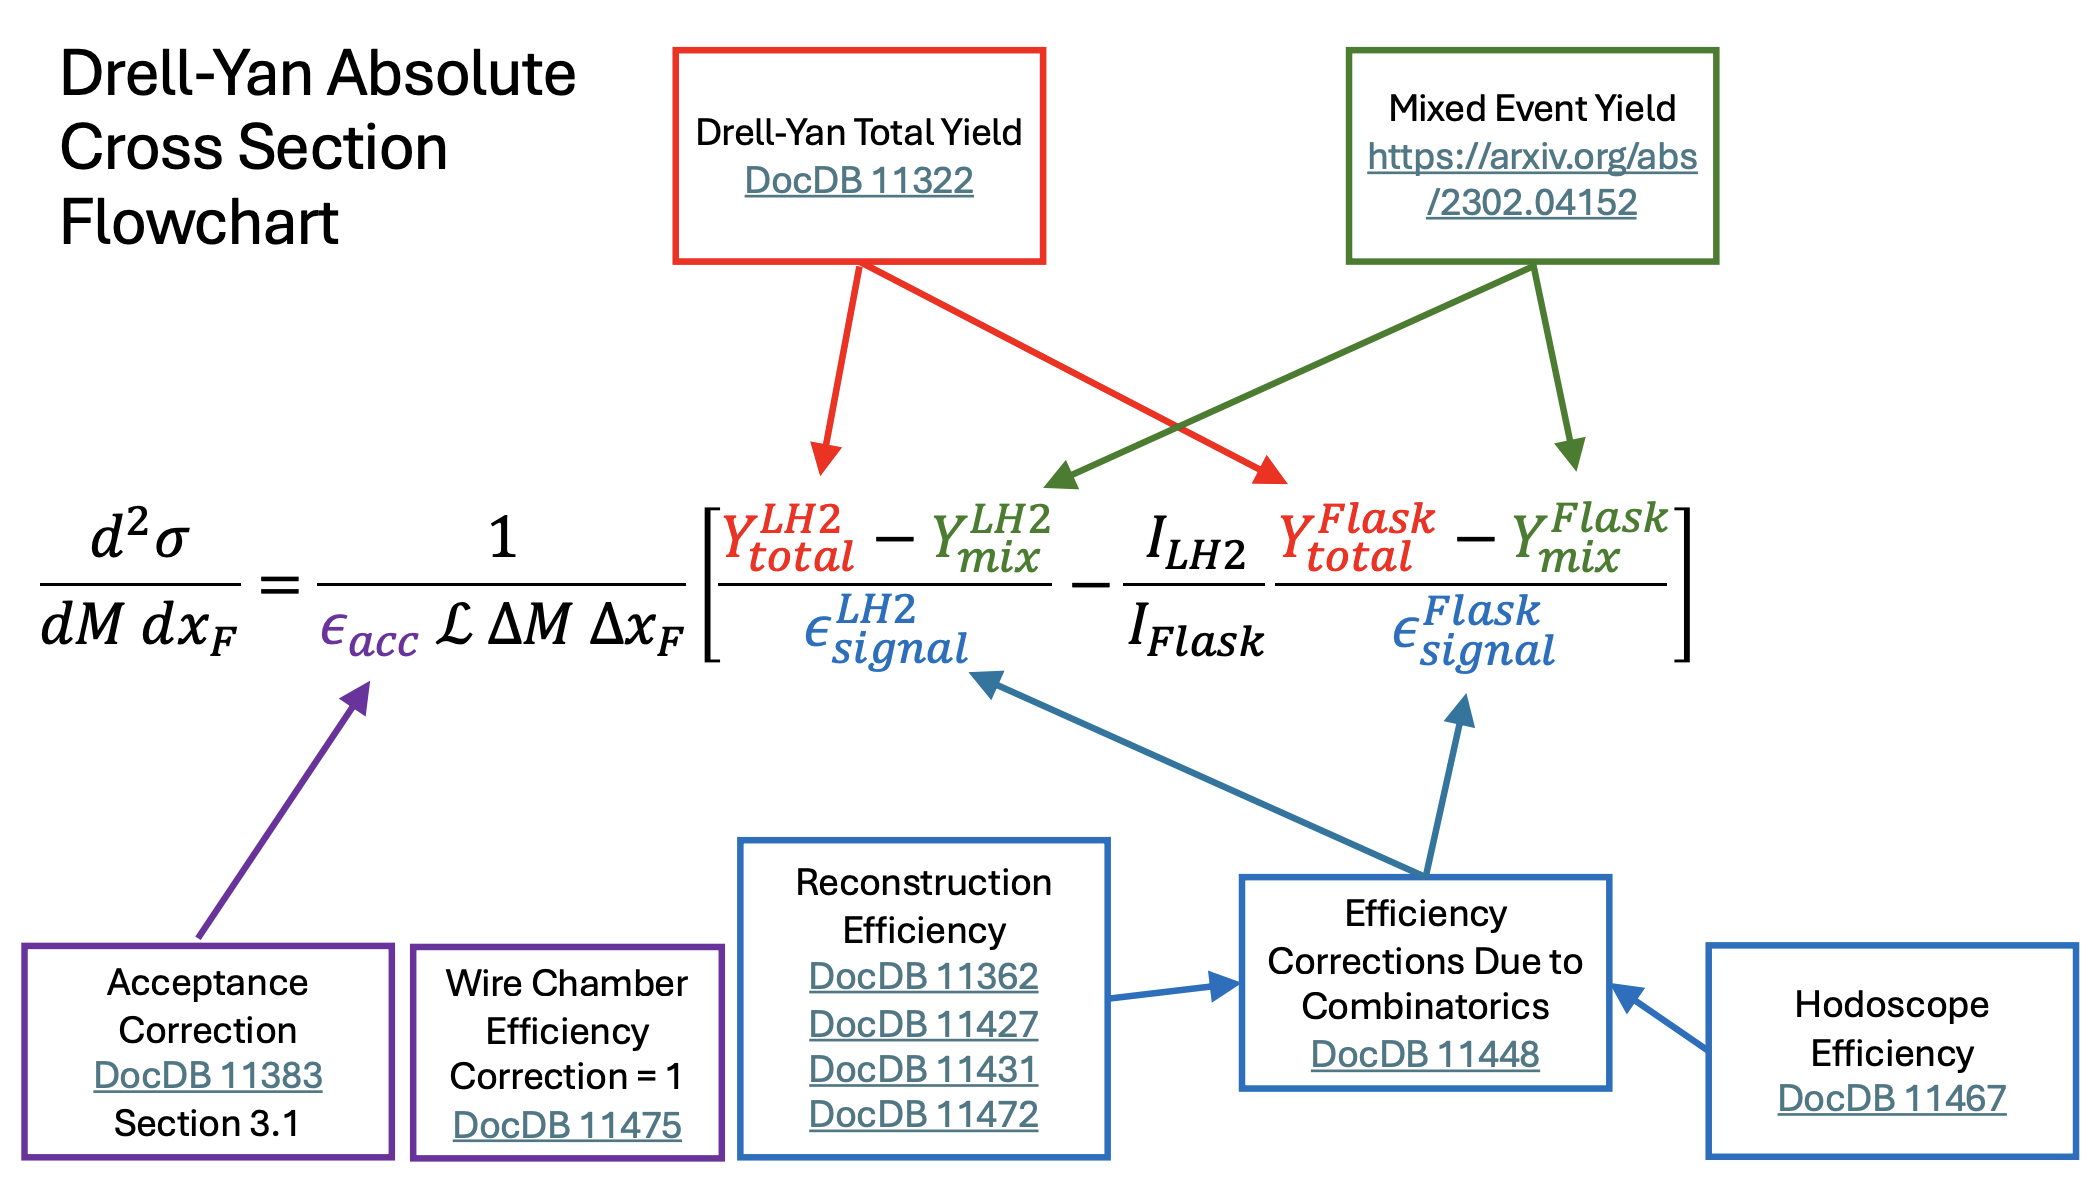
\includegraphics[width=\textwidth,height=0.8\textheight,keepaspectratio]{xsec_flowchart.png}
    \end{center}
\end{frame}

\begin{frame}{Uncertainties}
    \begin{center}
        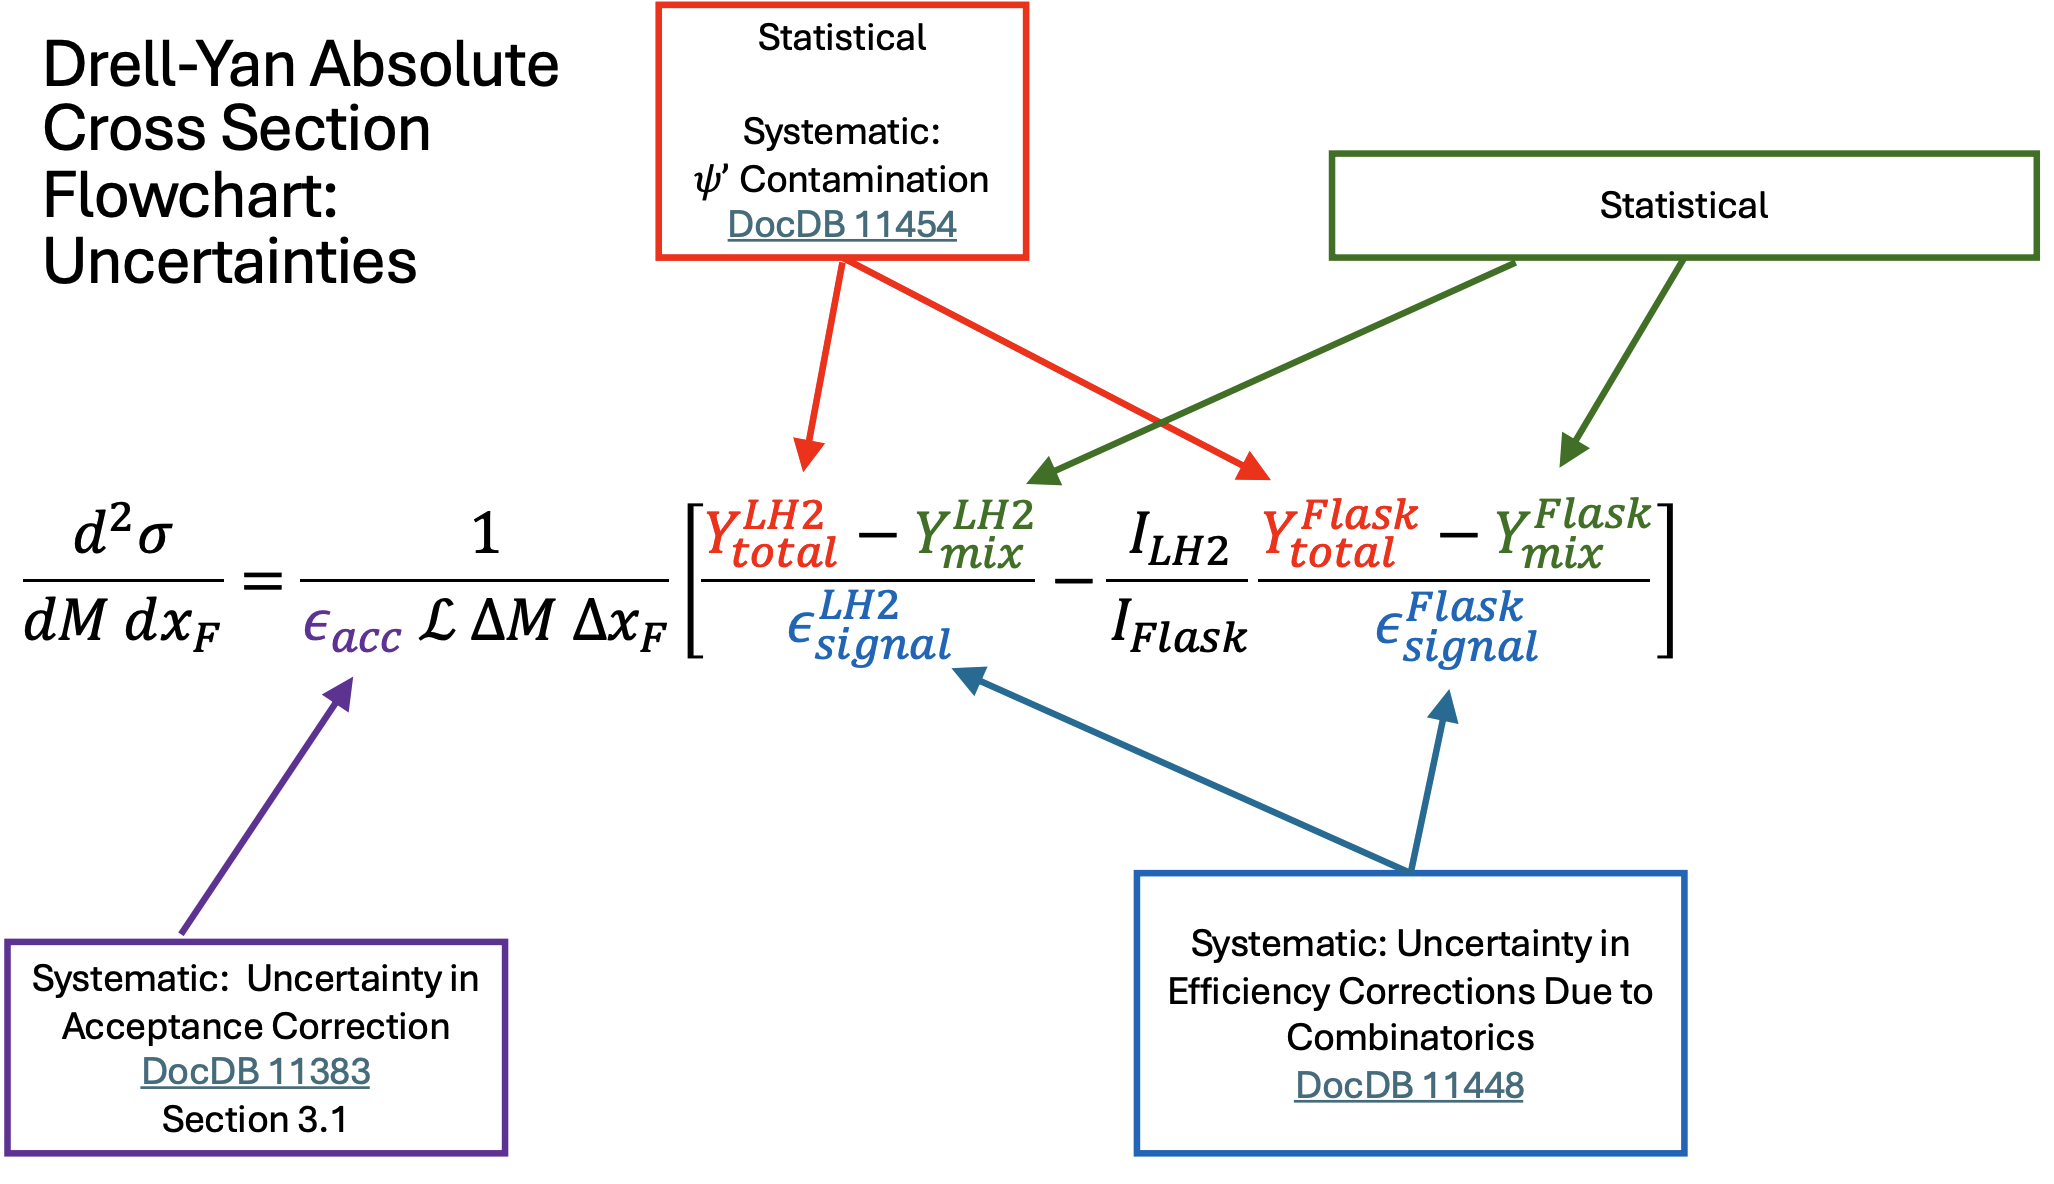
\includegraphics[width=\textwidth,height=0.8\textheight,keepaspectratio]{xsec_uncertainties.png}
    \end{center}
\end{frame}

\begin{frame}{Determination of $\epsilon_{\text{signal}}$}
    
\small
For a given target (LH2 or LD2 or Flask) and a given kinematic ($M, x_F, p_T$) bin, there will be $Y_{\text{total}}$ dimuons in the normal event stream and $Y_{\text{mix}}$ dimuons from the mixed event stream.

\vspace{0.2cm}
\begin{columns}[T]
    \begin{column}{0.65\textwidth}
        \begin{equation*}
            \langle \epsilon \rangle_{\text{total}}^{\text{hodo}} = \frac{1}{Y_{\text{total}}} \sum_{i=1}^{Y_{\text{total}}} \epsilon_i^{\text{hodo}}
        \end{equation*}
        \begin{equation*}
            \langle \epsilon \rangle_{\text{mix}}^{\text{hodo}} = \frac{1}{Y_{\text{mix}}} \sum_{j=1}^{Y_{\text{mix}}} \epsilon_j^{\text{hodo}}
        \end{equation*}
        \begin{equation*}
            \langle \epsilon \rangle_{\text{total}}^{\text{reco}} = \frac{1}{Y_{\text{total}}} \sum_{i=1}^{Y_{\text{total}}} \epsilon_i^{\text{reco}}
        \end{equation*}
        \begin{equation*}
            \langle \epsilon \rangle_{\text{mix}}^{\text{reco}} = \frac{1}{Y_{\text{mix}}} \sum_{j=1}^{Y_{\text{mix}}} \epsilon_j^{\text{reco}}
        \end{equation*}
    \end{column}
    \begin{column}{0.35\textwidth}
        \vspace{0.4cm}
        \scriptsize
        $\epsilon_{\text{hodo}} = [\epsilon_{st1}^x \epsilon_{st2}^x \epsilon_{st3}^x \epsilon_{st4}^x \epsilon_{st1}^y \epsilon_{st2}^y \epsilon_{st3}^y \epsilon_{st4}^y]_i$
        \vspace{0.4cm}
        
        $\delta\langle\epsilon\rangle_{\text{total}}^{\text{hodo}}$ and $\delta\langle\epsilon\rangle_{\text{mix}}^{\text{hodo}}$ are propagated from hodoscope paddle efficiencies.
        \vspace{0.6cm}
        
        $\epsilon^{\text{reco}}$ interpolated from $\epsilon(D1)$ function.
        \vspace{0.4cm}
        $\langle \epsilon \rangle_{\text{total}} = \langle \epsilon \rangle_{\text{total}}^{\text{hodo}} \langle \epsilon \rangle_{\text{total}}^{\text{reco}}$ \qquad $\langle \epsilon \rangle_{\text{mix}} = \langle \epsilon \rangle_{\text{mix}}^{\text{hodo}} \langle \epsilon \rangle_{\text{mix}}^{\text{reco}}$
        \vspace{0.4cm}\\
        $\delta\langle\epsilon\rangle_{\text{total}}^{\text{reco}}$ and $\delta\langle\epsilon\rangle_{\text{mix}}^{\text{reco}}$ include correlations\\
        \vspace{0.4cm}\\
        (See \href{https://seaquest-docdb.fnal.gov/cgi-bin/sso/ShowDocument?docid=11431}{DocDB 11431})
    \end{column}
\end{columns}

%\vspace{0.3cm}
\centering


%\vspace{0.2cm}
\begin{columns}[c]
    \begin{column}{0.65\textwidth}
        \begin{equation*}
            \epsilon_{\text{signal}} = \frac{\langle \epsilon \rangle_{\text{total}} Y_{\text{total}} - \langle \epsilon \rangle_{\text{mix}} Y_{\text{mix}}}{Y_{\text{total}} - Y_{\text{mix}}} \qquad \text{\href{https://seaquest-docdb.fnal.gov/cgi-bin/sso/ShowDocument?docid=11448}{DocDB 11448}}
        \end{equation*}
    \end{column}
    \begin{column}{0.35\textwidth}
        \scriptsize
        $\delta\epsilon_{\text{signal}}$ propagated from uncertainties in the six inputs.
    \end{column}
\end{columns}
\normalsize

\end{frame}

\begin{frame}{Y\_total\_LH2}
    \begin{center}
        
\includegraphics[width=\textwidth,height=0.8\textheight,keepaspectratio]{Y_total_LH2.pdf}
    \end{center}
\end{frame}

\begin{frame}{Y\_total\_LD2}
    \begin{center}
        
\includegraphics[width=\textwidth,height=0.8\textheight,keepaspectratio]{Y_total_LD2.pdf}
    \end{center}
\end{frame}

\begin{frame}{Y\_total\_Flask}
    \begin{center}
        
\includegraphics[width=\textwidth,height=0.8\textheight,keepaspectratio]{Y_total_Flask.pdf}
    \end{center}
\end{frame}

\begin{frame}{Y\_mix\_LH2}
    \begin{center}
        
\includegraphics[width=\textwidth,height=0.8\textheight,keepaspectratio]{Y_mix_LH2.pdf}
    \end{center}
\end{frame}

\begin{frame}{Y\_mix\_LD2}
    \begin{center}
        
\includegraphics[width=\textwidth,height=0.8\textheight,keepaspectratio]{Y_mix_LD2.pdf}
    \end{center}
\end{frame}

\begin{frame}{Y\_mix\_Flask}
    \begin{center}
        
\includegraphics[width=\textwidth,height=0.8\textheight,keepaspectratio]{Y_mix_Flask.pdf}
    \end{center}
\end{frame}

\begin{frame}{E\_total\_reco\_LH2}
    \begin{center}
        
\includegraphics[width=\textwidth,height=0.8\textheight,keepaspectratio]{E_total_reco_LH2.pdf}
    \end{center}
\end{frame}

\begin{frame}{E\_total\_reco\_LD2}
    \begin{center}
        
\includegraphics[width=\textwidth,height=0.8\textheight,keepaspectratio]{E_total_reco_LD2.pdf}
    \end{center}
\end{frame}

\begin{frame}{E\_total\_reco\_Flask}
    \begin{center}
        
\includegraphics[width=\textwidth,height=0.8\textheight,keepaspectratio]{E_total_reco_Flask.pdf}
    \end{center}
\end{frame}

\begin{frame}{E\_mix\_reco\_LH2}
    \begin{center}
        
\includegraphics[width=\textwidth,height=0.8\textheight,keepaspectratio]{E_mix_reco_LH2.pdf}
    \end{center}
\end{frame}

\begin{frame}{E\_mix\_reco\_LD2}
    \begin{center}
        
\includegraphics[width=\textwidth,height=0.8\textheight,keepaspectratio]{E_mix_reco_LD2.pdf}
    \end{center}
\end{frame}

\begin{frame}{E\_mix\_reco\_Flask}
    \begin{center}
        
\includegraphics[width=\textwidth,height=0.8\textheight,keepaspectratio]{E_mix_reco_Flask.pdf}
    \end{center}
\end{frame}

\begin{frame}{E\_total\_hodo\_LH2}
    \begin{center}
        
\includegraphics[width=\textwidth,height=0.8\textheight,keepaspectratio]{E_total_hodo_LH2.pdf}
    \end{center}
\end{frame}

\begin{frame}{E\_total\_hodo\_LD2}
    \begin{center}
        
\includegraphics[width=\textwidth,height=0.8\textheight,keepaspectratio]{E_total_hodo_LD2.pdf}
    \end{center}
\end{frame}

\begin{frame}{E\_total\_hodo\_Flask}
    \begin{center}
        
\includegraphics[width=\textwidth,height=0.8\textheight,keepaspectratio]{E_total_hodo_Flask.pdf}
    \end{center}
\end{frame}

\begin{frame}{E\_mix\_hodo\_LH2}
    \begin{center}
        
\includegraphics[width=\textwidth,height=0.8\textheight,keepaspectratio]{E_mix_hodo_LH2.pdf}
    \end{center}
\end{frame}

\begin{frame}{E\_mix\_hodo\_LD2}
    \begin{center}
        
\includegraphics[width=\textwidth,height=0.8\textheight,keepaspectratio]{E_mix_hodo_LD2.pdf}
    \end{center}
\end{frame}

\begin{frame}{E\_mix\_hodo\_Flask}
    \begin{center}
        
\includegraphics[width=\textwidth,height=0.8\textheight,keepaspectratio]{E_mix_hodo_Flask.pdf}
    \end{center}
\end{frame}

\begin{frame}{E\_total\_final\_LH2}
    \begin{center}
        
\includegraphics[width=\textwidth,height=0.8\textheight,keepaspectratio]{E_total_final_LH2.pdf}
    \end{center}
\end{frame}

\begin{frame}{E\_total\_final\_LD2}
    \begin{center}
        
\includegraphics[width=\textwidth,height=0.8\textheight,keepaspectratio]{E_total_final_LD2.pdf}
    \end{center}
\end{frame}

\begin{frame}{E\_total\_final\_Flask}
    \begin{center}
        
\includegraphics[width=\textwidth,height=0.8\textheight,keepaspectratio]{E_total_final_Flask.pdf}
    \end{center}
\end{frame}

\begin{frame}{E\_mix\_final\_LH2}
    \begin{center}
        
\includegraphics[width=\textwidth,height=0.8\textheight,keepaspectratio]{E_mix_final_LH2.pdf}
    \end{center}
\end{frame}

\begin{frame}{E\_mix\_final\_LD2}
    \begin{center}
        
\includegraphics[width=\textwidth,height=0.8\textheight,keepaspectratio]{E_mix_final_LD2.pdf}
    \end{center}
\end{frame}

\begin{frame}{E\_mix\_final\_Flask}
    \begin{center}
        
\includegraphics[width=\textwidth,height=0.8\textheight,keepaspectratio]{E_mix_final_Flask.pdf}
    \end{center}
\end{frame}

\begin{frame}{E\_final\_signal\_LH2}
    \begin{center}
        
\includegraphics[width=\textwidth,height=0.8\textheight,keepaspectratio]{E_final_signal_LH2.pdf}
    \end{center}
\end{frame}

\begin{frame}{E\_final\_signal\_LD2}
    \begin{center}
        
\includegraphics[width=\textwidth,height=0.8\textheight,keepaspectratio]{E_final_signal_LD2.pdf}
    \end{center}
\end{frame}

\begin{frame}{E\_final\_signal\_Flask}
    \begin{center}
        
\includegraphics[width=\textwidth,height=0.8\textheight,keepaspectratio]{E_final_signal_Flask.pdf}
    \end{center}
\end{frame}

\begin{frame}{Y\_corrected\_LH2}
    \begin{center}
        
\includegraphics[width=\textwidth,height=0.8\textheight,keepaspectratio]{Y_corrected_LH2.pdf}
    \end{center}
\end{frame}

\begin{frame}{Y\_corrected\_LD2}
    \begin{center}
        
\includegraphics[width=\textwidth,height=0.8\textheight,keepaspectratio]{Y_corrected_LD2.pdf}
    \end{center}
\end{frame}

\begin{frame}{Y\_corrected\_Flask}
    \begin{center}
        
\includegraphics[width=\textwidth,height=0.8\textheight,keepaspectratio]{Y_corrected_Flask.pdf}
    \end{center}
\end{frame}

\begin{frame}{Y\_corrected\_Subtracted\_LH2}
    \begin{center}
        
\includegraphics[width=\textwidth,height=0.8\textheight,keepaspectratio]{Y_corrected_Subtracted_LH2.pdf}
    \end{center}
\end{frame}

\begin{frame}{Y\_corrected\_Subtracted\_LD2}
    \begin{center}
        
\includegraphics[width=\textwidth,height=0.8\textheight,keepaspectratio]{Y_corrected_Subtracted_LD2.pdf}
    \end{center}
\end{frame}

\begin{frame}{CrossSection\_LH2\_geom\_vs\_pT\_with\_logo}
    \begin{center}
        
\includegraphics[width=\textwidth,height=0.8\textheight,keepaspectratio]{CrossSection_LH2_geom_vs_pT_with_logo.pdf}
    \end{center}
\end{frame}

\begin{frame}{CrossSection\_LH2\_true\_pt\_vs\_pT\_with\_logo}
    \begin{center}
        
\includegraphics[width=\textwidth,height=0.8\textheight,keepaspectratio]{CrossSection_LH2_true_pt_vs_pT_with_logo.pdf}
    \end{center}
\end{frame}

\begin{frame}{CrossSection\_LD2\_geom\_vs\_pT\_with\_logo}
    \begin{center}
        
\includegraphics[width=\textwidth,height=0.8\textheight,keepaspectratio]{CrossSection_LD2_geom_vs_pT_with_logo.pdf}
    \end{center}
\end{frame}

\begin{frame}{CrossSection\_LD2\_true\_pt\_vs\_pT\_with\_logo}
    \begin{center}
        
\includegraphics[width=\textwidth,height=0.8\textheight,keepaspectratio]{CrossSection_LD2_true_pt_vs_pT_with_logo.pdf}
    \end{center}
\end{frame}

\begin{frame}{CrossSection\_Ratio\_pd\_2pp\_vs\_pT\_geom\_with\_logo}
    \begin{center}
        
\includegraphics[width=\textwidth,height=0.8\textheight,keepaspectratio]{CrossSection_Ratio_pd_2pp_vs_pT_geom_with_logo.pdf}
    \end{center}
\end{frame}

\begin{frame}{CrossSection\_Ratio\_pd\_2pp\_vs\_pT\_true\_pt\_with\_logo}
    \begin{center}
        
\includegraphics[width=\textwidth,height=0.8\textheight,keepaspectratio]{CrossSection_Ratio_pd_2pp_vs_pT_true_pt_with_logo.pdf}
    \end{center}
\end{frame}

\begin{frame}{Combined\_XSec\_Ratio\_vs\_pT\_geom}
    \begin{center}
        
\includegraphics[width=\textwidth,height=0.8\textheight,keepaspectratio]{Combined_XSec_Ratio_vs_pT_geom.pdf}
    \end{center}
\end{frame}

\begin{frame}{Combined\_XSec\_Ratio\_vs\_pT\_true\_pt}
    \begin{center}
        
\includegraphics[width=\textwidth,height=0.8\textheight,keepaspectratio]{Combined_XSec_Ratio_vs_pT_true_pt.pdf}
    \end{center}
\end{frame}

\begin{frame}{Next Steps}
    
\begin{itemize}
    \setlength{\itemsep}{1em}
    \item Need to work on unfolding (work on progress).
    \item We are planning to present these preliminary plots during the upcoming APS DPF meeting.
    \item Another set of cross-section plots will be generated after integrating run 5 data.
\end{itemize}

\end{frame}

\appendix

\begin{frame}
    \vfill
    \centering
    \begin{beamercolorbox}[sep=8pt,center,shadow=true,rounded=true]{title}
        \usebeamerfont{title}Backup Slides\par%
    \end{beamercolorbox}
    \vfill
\end{frame}

\begin{frame}{Cross-Section LD2 $0.00 \le x_{F} < 0.05$}
    \begin{center}
        
\includegraphics[width=\textwidth,height=0.8\textheight,keepaspectratio]{CrossSection_LD2_xF_0.00_0.05_GeoCenter_with_logo.pdf}
    \end{center}
\end{frame}

\begin{frame}{Cross-Section LD2 $0.05 \le x_{F} < 0.10$}
    \begin{center}
        
\includegraphics[width=\textwidth,height=0.8\textheight,keepaspectratio]{CrossSection_LD2_xF_0.05_0.10_GeoCenter_with_logo.pdf}
    \end{center}
\end{frame}

\begin{frame}{Cross-Section LD2 $0.10 \le x_{F} < 0.15$}
    \begin{center}
        
\includegraphics[width=\textwidth,height=0.8\textheight,keepaspectratio]{CrossSection_LD2_xF_0.10_0.15_GeoCenter_with_logo.pdf}
    \end{center}
\end{frame}

\begin{frame}{Cross-Section LD2 $0.15 \le x_{F} < 0.20$}
    \begin{center}
        
\includegraphics[width=\textwidth,height=0.8\textheight,keepaspectratio]{CrossSection_LD2_xF_0.15_0.20_GeoCenter_with_logo.pdf}
    \end{center}
\end{frame}

\begin{frame}{Cross-Section LD2 $0.20 \le x_{F} < 0.25$}
    \begin{center}
        
\includegraphics[width=\textwidth,height=0.8\textheight,keepaspectratio]{CrossSection_LD2_xF_0.20_0.25_GeoCenter_with_logo.pdf}
    \end{center}
\end{frame}

\begin{frame}{Cross-Section LD2 $0.25 \le x_{F} < 0.30$}
    \begin{center}
        
\includegraphics[width=\textwidth,height=0.8\textheight,keepaspectratio]{CrossSection_LD2_xF_0.25_0.30_GeoCenter_with_logo.pdf}
    \end{center}
\end{frame}

\begin{frame}{Cross-Section LD2 $0.30 \le x_{F} < 0.35$}
    \begin{center}
        
\includegraphics[width=\textwidth,height=0.8\textheight,keepaspectratio]{CrossSection_LD2_xF_0.30_0.35_GeoCenter_with_logo.pdf}
    \end{center}
\end{frame}

\begin{frame}{Cross-Section LD2 $0.35 \le x_{F} < 0.40$}
    \begin{center}
        
\includegraphics[width=\textwidth,height=0.8\textheight,keepaspectratio]{CrossSection_LD2_xF_0.35_0.40_GeoCenter_with_logo.pdf}
    \end{center}
\end{frame}

\begin{frame}{Cross-Section LD2 $0.40 \le x_{F} < 0.45$}
    \begin{center}
        
\includegraphics[width=\textwidth,height=0.8\textheight,keepaspectratio]{CrossSection_LD2_xF_0.40_0.45_GeoCenter_with_logo.pdf}
    \end{center}
\end{frame}

\begin{frame}{Cross-Section LD2 $0.45 \le x_{F} < 0.50$}
    \begin{center}
        
\includegraphics[width=\textwidth,height=0.8\textheight,keepaspectratio]{CrossSection_LD2_xF_0.45_0.50_GeoCenter_with_logo.pdf}
    \end{center}
\end{frame}

\begin{frame}{Cross-Section LD2 $0.50 \le x_{F} < 0.55$}
    \begin{center}
        
\includegraphics[width=\textwidth,height=0.8\textheight,keepaspectratio]{CrossSection_LD2_xF_0.50_0.55_GeoCenter_with_logo.pdf}
    \end{center}
\end{frame}

\begin{frame}{Cross-Section LD2 $0.55 \le x_{F} < 0.60$}
    \begin{center}
        
\includegraphics[width=\textwidth,height=0.8\textheight,keepaspectratio]{CrossSection_LD2_xF_0.55_0.60_GeoCenter_with_logo.pdf}
    \end{center}
\end{frame}

\begin{frame}{Cross-Section LD2 $0.60 \le x_{F} < 0.65$}
    \begin{center}
        
\includegraphics[width=\textwidth,height=0.8\textheight,keepaspectratio]{CrossSection_LD2_xF_0.60_0.65_GeoCenter_with_logo.pdf}
    \end{center}
\end{frame}

\begin{frame}{Cross-Section LD2 $0.65 \le x_{F} < 0.70$}
    \begin{center}
        
\includegraphics[width=\textwidth,height=0.8\textheight,keepaspectratio]{CrossSection_LD2_xF_0.65_0.70_GeoCenter_with_logo.pdf}
    \end{center}
\end{frame}

\begin{frame}{Cross-Section LD2 $0.70 \le x_{F} < 0.75$}
    \begin{center}
        
\includegraphics[width=\textwidth,height=0.8\textheight,keepaspectratio]{CrossSection_LD2_xF_0.70_0.75_GeoCenter_with_logo.pdf}
    \end{center}
\end{frame}

\begin{frame}{Cross-Section LD2 $0.75 \le x_{F} < 0.80$}
    \begin{center}
        
\includegraphics[width=\textwidth,height=0.8\textheight,keepaspectratio]{CrossSection_LD2_xF_0.75_0.80_GeoCenter_with_logo.pdf}
    \end{center}
\end{frame}

\begin{frame}{Cross-Section LH2 $0.00 \le x_{F} < 0.05$}
    \begin{center}
        
\includegraphics[width=\textwidth,height=0.8\textheight,keepaspectratio]{CrossSection_LH2_xF_0.00_0.05_GeoCenter_with_logo.pdf}
    \end{center}
\end{frame}

\begin{frame}{Cross-Section LH2 $0.05 \le x_{F} < 0.10$}
    \begin{center}
        
\includegraphics[width=\textwidth,height=0.8\textheight,keepaspectratio]{CrossSection_LH2_xF_0.05_0.10_GeoCenter_with_logo.pdf}
    \end{center}
\end{frame}

\begin{frame}{Cross-Section LH2 $0.10 \le x_{F} < 0.15$}
    \begin{center}
        
\includegraphics[width=\textwidth,height=0.8\textheight,keepaspectratio]{CrossSection_LH2_xF_0.10_0.15_GeoCenter_with_logo.pdf}
    \end{center}
\end{frame}

\begin{frame}{Cross-Section LH2 $0.15 \le x_{F} < 0.20$}
    \begin{center}
        
\includegraphics[width=\textwidth,height=0.8\textheight,keepaspectratio]{CrossSection_LH2_xF_0.15_0.20_GeoCenter_with_logo.pdf}
    \end{center}
\end{frame}

\begin{frame}{Cross-Section LH2 $0.20 \le x_{F} < 0.25$}
    \begin{center}
        
\includegraphics[width=\textwidth,height=0.8\textheight,keepaspectratio]{CrossSection_LH2_xF_0.20_0.25_GeoCenter_with_logo.pdf}
    \end{center}
\end{frame}

\begin{frame}{Cross-Section LH2 $0.25 \le x_{F} < 0.30$}
    \begin{center}
        
\includegraphics[width=\textwidth,height=0.8\textheight,keepaspectratio]{CrossSection_LH2_xF_0.25_0.30_GeoCenter_with_logo.pdf}
    \end{center}
\end{frame}

\begin{frame}{Cross-Section LH2 $0.30 \le x_{F} < 0.35$}
    \begin{center}
        
\includegraphics[width=\textwidth,height=0.8\textheight,keepaspectratio]{CrossSection_LH2_xF_0.30_0.35_GeoCenter_with_logo.pdf}
    \end{center}
\end{frame}

\begin{frame}{Cross-Section LH2 $0.35 \le x_{F} < 0.40$}
    \begin{center}
        
\includegraphics[width=\textwidth,height=0.8\textheight,keepaspectratio]{CrossSection_LH2_xF_0.35_0.40_GeoCenter_with_logo.pdf}
    \end{center}
\end{frame}

\begin{frame}{Cross-Section LH2 $0.40 \le x_{F} < 0.45$}
    \begin{center}
        
\includegraphics[width=\textwidth,height=0.8\textheight,keepaspectratio]{CrossSection_LH2_xF_0.40_0.45_GeoCenter_with_logo.pdf}
    \end{center}
\end{frame}

\begin{frame}{Cross-Section LH2 $0.45 \le x_{F} < 0.50$}
    \begin{center}
        
\includegraphics[width=\textwidth,height=0.8\textheight,keepaspectratio]{CrossSection_LH2_xF_0.45_0.50_GeoCenter_with_logo.pdf}
    \end{center}
\end{frame}

\begin{frame}{Cross-Section LH2 $0.50 \le x_{F} < 0.55$}
    \begin{center}
        
\includegraphics[width=\textwidth,height=0.8\textheight,keepaspectratio]{CrossSection_LH2_xF_0.50_0.55_GeoCenter_with_logo.pdf}
    \end{center}
\end{frame}

\begin{frame}{Cross-Section LH2 $0.55 \le x_{F} < 0.60$}
    \begin{center}
        
\includegraphics[width=\textwidth,height=0.8\textheight,keepaspectratio]{CrossSection_LH2_xF_0.55_0.60_GeoCenter_with_logo.pdf}
    \end{center}
\end{frame}

\begin{frame}{Cross-Section LH2 $0.60 \le x_{F} < 0.65$}
    \begin{center}
        
\includegraphics[width=\textwidth,height=0.8\textheight,keepaspectratio]{CrossSection_LH2_xF_0.60_0.65_GeoCenter_with_logo.pdf}
    \end{center}
\end{frame}

\begin{frame}{Cross-Section LH2 $0.65 \le x_{F} < 0.70$}
    \begin{center}
        
\includegraphics[width=\textwidth,height=0.8\textheight,keepaspectratio]{CrossSection_LH2_xF_0.65_0.70_GeoCenter_with_logo.pdf}
    \end{center}
\end{frame}

\begin{frame}{Cross-Section LH2 $0.70 \le x_{F} < 0.75$}
    \begin{center}
        
\includegraphics[width=\textwidth,height=0.8\textheight,keepaspectratio]{CrossSection_LH2_xF_0.70_0.75_GeoCenter_with_logo.pdf}
    \end{center}
\end{frame}

\begin{frame}{Cross-Section LH2 $0.75 \le x_{F} < 0.80$}
    \begin{center}
        
\includegraphics[width=\textwidth,height=0.8\textheight,keepaspectratio]{CrossSection_LH2_xF_0.75_0.80_GeoCenter_with_logo.pdf}
    \end{center}
\end{frame}

\end{document}
